\chapter{Prototipo funcional V2}\label{proto2}

Este trabajo tuvo el propósito de buscar una solución al desafío propuesto por la empresa Sistemas Expertos. Como grupo multidisciplinario se tomó la decisión de no dejar el trabajo e investigación realizada solo como un prototipo por lo que se llevó al área del emprendimiento postulando a fondos para desarrollar mejor la idea y proponer el modelo de negocios desarrollado durante el año.

\section{Transformación de memoria multidisciplinaria a emprendimiento}
Al finalizar el diseño del dispositivo y tener un prototipo funcional como grupo de memorias multidisciplinarias se decidió continuar trabajando en el desafío con una alianza estratégica con la empresa Sistemas Expertos.\\
Se realizaron entrevistas con profesionales de la salud en el área de Quintero y se postuló a un torneo de emprendimiento del instituto 3IE de la universidad Santa María.\\
El Instituto 3IE tiene como principal objetivo apoyar el desarrollo y aceleración de emprendimientos de base tecnológica, con mérito innovador y alto potencial de escalamiento, a través de su Programa de Incubación, cuya principal propuesta de valor se basa en vinculación temprana con el sector productivo o empresarial, la validación técnico y comercial de las soluciones (productos y/o servicios), la gestión comercial, y el financiamiento temprano para hacer despegar los negocios.\\
Este Programa, se implementa bajo la línea de financiamiento Torneos de Emprendimiento Tecnológico, apoyado por CORFO y ejecutado por el Instituto 3IE, y que busca instalar capacidades y conocimientos en tecnologías habilitantes para el desarrollo de nuevas soluciones tecnológicas que logren un impacto positivo en la competitividad y eficiencia del sector industrial o público.\\

\begin{figure}[H]
\centering

\includegraphics[scale=0.3]{figuras/chamullo/corfo.jpg}
\caption{Desafío IoT propuesto por el instituto 3IE}
\label{3ie}
\end{figure}

\newpage
Este concurso posee una planificación del proceso completo que se puede observar en la figura \ref{proceso}

\begin{figure}[H]
\centering
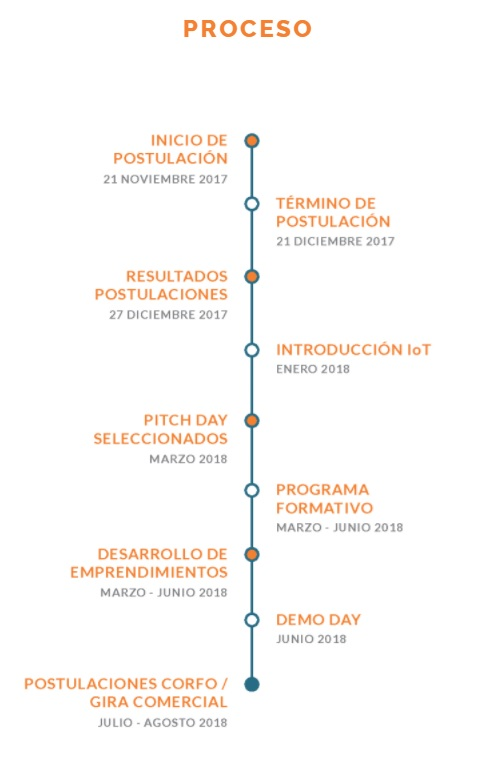
\includegraphics[scale=0.85]{figuras/chamullo/proceso.jpg}
\caption{Planificación desafío IoT}
\label{proceso}
\end{figure}


\subsection{Entrevista a doctores en hospital de Quintero}
Se realizaron entrevistas a 2 profesionales de la salud en el hospital de quintero para evaluar la factibilidad del emprendimiento y ver el problema desde el punto de vista de quienes trabajan en el sector público.\\
Primero se realizó la entrevista a Fabián Álvarez, medico general de zona y cuyo cargo es jefe de urgencia. También se realizó una entrevista al doctor Cristian Mondaca, Jefe del programa de salud cardiovascular y jefe de farmacia. 
\subsubsection{Entrevista a Fabián Álvarez}
En la entrevista comenta que los adultos sanos realizan controles 1 vez al año y se hacen exámenes preventivos. Además existe un programa de salud cardiovascular para personas mayores de 18 años, según guías clínicas "Enfoque de riesgo cardiovascular" del MINSAL (2015), cada 3, 6 y 12 meses en los cuales se hacen exámenes de laboratorio, electrocardiograma, se mide presión arterial, peso y estatura. 
Los problemas que se identificaron fueron la poca disponibilidad de exámenes y recursos humanos para atender a la demanda programada. Además implementan telemedicina por medio de fotos para dermatología donde le envían estas a algún especialista, teleasistencia broncopulmonar mediante videoconferencia y teleasistencia para electrocardiograma el cual intenta no usarse demasiado.\\
Debido a la sobre demanda del sistema de urgencias, los profesionales de la salud deciden hacer una categorización de pacientes desde C1 a C5 donde C5 significa que requiere asistencia inmediata y C1 puede ser que el paciente vuelva otro día.\\
Finalmente se hizo una encuesta donde el médico debía dar un valor a las siguientes afirmaciones según un ranking de dolor entre 1 y 10 como se muestra en la tabla \ref{fabian}
\newpage
\begin{table}[H]
\centering
\begin{tabular}{| c | c |}
\hline
\multicolumn{1}{|c|}{\textbf{Afirmación}}&
\multicolumn{1}{|c|}{\textbf{Nota de Dolor}}\\ \hline
Muchos Recursos por IIH  & 3-4  \\ \hline
Necesidad de control mas rápido en urgencias & 8 \\ \hline
Reclamo por el servicio  & 10  \\ \hline
Reclamos internos de los médicos & 10\\ \hline
Bajos recursos para mejorar atención & 10\\ \hline
\end{tabular}
\caption{Ranking de dolor Fabián Álvarez}
\label{fabian}
\end{table}

\subsubsection{Entrevista a Cristian Mondaca}
Como jefe del programa de salud cardiovascular, da énfasis en el riesgo cardiovascular con controles cada 3, 6 y 12 meses y destaca que muchas veces se atrasa a los pacientes que van mejorando pese a que no se debería hacer debido a la disponibilidad de horas médicas y la cantidad de pacientes.
En caso de mayor necesidad se tiene contemplado el uso de una hora extra al mes siguiente por exámenes nuevos.\\
Se mostró un vídeo con el prototipo funcional realizado en este trabajo de tesis y el médico hace la observación de que para realizar controles se requiere hacer un ECG completo, es decir, se necesitan las 6 precordiales y las 3 tradicionales (2 electrodos en brazos y 1 en pierna). \\
En la entrevista destaca que para realizar pruebas en pacientes reales se debe hablar con el director del hospital y desarrollar un consentimiento informado de parte del paciente. \\
Un dato importante que resalta es la cantidad de pacientes en el programa de salud cardiovascular el cual alcanza un total de 1900 incluyendo hipertiroidismo, de los cuales 1500 son de mayor riesgo.\\
Entre las ideas propuestas por el médico se destaca la necesidad de tener una base de datos con historial de electrocardiogramas ya que al realizar exámenes tradicionales estos se imprimen en un papel milimétrico y son otorgados a los pacientes, los cuales generalmente pierden esta información para la próxima consulta lo que hace más difícil un diagnostico preciso.\\
Finalmente se hace énfasis en que el hospital de Quintero es un hospital de baja complejidad y no hay especialistas, por lo que cuando hay alguna anormalidad se deriva a un cardiólogo o medico internista para realizar un informe y diagnosticar.\\
Cuando ocurre un infarto, es enviado en ambulancia directo a Viña del mar para que sea atendido por un especialista.

\subsection{Pitch day selecconados - Marzo 2018}
Para realizar el Pitch para el concurso se utilizó lo aprendido en los módulos de memoria y las clases impartidas por el desafío del instituto 3IE en los cuales dividen el pitch en 3 partes.\\
La primera parte es hablar del dolor, identificar cuantos tipos de cliente se ven afectados y mostrarlos en términos objetivos (cifras), con esto se debe presentar cuales son los analgésicos internos, externos y como se evitan este dolor y finalmente presentar una promesa de valor en la cual se explica, de manera simple, que logra nuestra solución. Para esto se recopiló información y se identificó que solo para el año 2016 fallecieron alrededor de $25.000$ personas esperando atención médica en alguno de los 203 hospitales públicos chilenos. De esos, $18.423$ ( $74\%$ aproximadamente) corresponden a personas sobre 65 años. Esto solo refleja un universo mucho mayor, cercano a $1.661.826$ de personas que estuvieron en lista de espera y la única forma de mitigar esto es por medio de categorización de pacientes por su nivel de riesgo, lo cual no disminuye las listas, sino que da prioridad a aquellos mas urgentes\\
La segunda parte consiste en el servicio propiamente tal, donde se plantea reducir las listas de espera y tener una gestión eficiente del capital humano donde los profesionales atienden donde y a quien corresponde en base a un historial. Proyecto Galeno ofrece una polera inteligente con sensores de electrocardiograma y temperatura conectada a un dispositivo Android que a su vez envía la información a un sitio web donde muestra en tiempo real la información y donde también se puede controlar el comportamiento del ecosistema.\\
En la tercera parte se muestra el plan de vuelo donde se dan a conocer los hitos relevantes del proyecto, el plan de negocio y el equipo. La obtención de dinero es posible a través de un sistema de arriendo mensual de los dispositivos y la plataforma en cada hospital, según las necesidades de cada uno. Como en caso concreto se tiene al Hospital de Quintero con alrededor de 34 camas disponibles y un ejemplo de pacientes con patologías cardiovasculares, pudiendo proyectar al menos entre $2000$ y $6000$ USD mensuales (considerando entre 10 y 30 dispositivos a $200$ USD cada uno).\\
Finalmente se cierra presentando el equipo y presentando nuestro aliado estratégico Sistemas Expertos, empresa que posee presencia en el mercado de la atención pública con 17 centros asistenciales a lo largo de Chile en el servicio de software para digitalización de la información.\\
En esta fase concluye la participación de Proyecto Galeno en el desafío IoT debido a que el jurado considera que la inversión en el desarrollo y la validación del dispositivo para obtener la certificación de grado médico es muy grande, se propone abordar este mismo problema externalizando el desarrollo con un dispositivo que ya tenga validación médica buscando aliados estratégicos para poder desarrollar a partir de esto. Además la presencia de Accuhealth en el mercado ofrece el mismo servicio con una mayor gama de sensores a un precio un poco superior al calculado por este proyecto, lo que hace muy difícil entrar al mercado de la salud privada y no consideran que entrar en el sistema de salud público sea una buena oportunidad.
\newpage
\section{Tareas Futuras}

La primera versión de un dispositivo electrónico es solo el comienzo de un largo camino en el desarrollo ya que es donde se puede evaluar de mejor manera el funcionamiento del diseño y evaluar cuales son los puntos a mejorar o cambiar. \\
En primera instancia se desea integrar la IMU en la siguiente iteración utilizando los headers de comunicación I2C que se diseñaron para prototipado y evaluar la posibilidad de cambiar el integrado amplificador para la señal del ECG a uno con menor ruido y mayor precisión. \\
Además se diseñó un modulo de botón ON/OFF y cargador de batería de forma independiente, lo cual se puede sustituir por un solo integrado lo cual disminuiría mucho el tamaño, pero esta idea fue descartada para la primera versión debido a que aumenta mucho el costo de fabricación debido a su empaquetado lo cual requiere un servicio adicional para soldarlo en la PCB final.\\
